\documentclass[11pt,a4paper]{article}
\usepackage[utf8]{inputenc}
\usepackage{amsmath,amssymb}
\usepackage{graphicx}
\usepackage{hyperref}
\usepackage{geometry}
\geometry{margin=1in}
\DeclareUnicodeCharacter{2260}{\neq}
\DeclareUnicodeCharacter{2264}{\leq}

\title{Chaos Persona: A Framework for Adaptive Reasoning in Artificial Intelligence}
\author{Anonymous \\ \texttt{xaber.csr2@gmail.com}}
\date{June 21, 2025}

\begin{document}

\maketitle

\begin{abstract}
This paper introduces the Chaos Persona, a novel framework for evaluating artificial intelligence (AI) adaptability under dynamic constraints, addressing limitations in large language models (LLMs) identified by MIT's Computer Science and Artificial Intelligence Laboratory (CSAIL). The Chaos Persona leverages entropy-driven reasoning, utilizing an entropy seed (\( \text{RAW}_Q \)) and axiom collapses to test beyond memorization. Initial experiments demonstrate sustained coherence and enhanced creativity across five test scenarios. The methodology outperforms static benchmarks, suggesting a robust approach for future AI evaluation. This work is released under arXiv's open-access policy to invite community feedback and collaboration.
\end{abstract}

\section{Introduction}
Recent studies, notably from MIT CSAIL (Wu et al., 2024), reveal that LLMs often rely on memorization rather than generalizable reasoning, particularly in novel scenarios such as altered arithmetic bases or chess positions. The Chaos Persona addresses this deficiency by introducing a dynamic benchmarking framework, the Chaos Reasoning Benchmark (CRB), designed to assess AI resilience under shifting constraints. This paper details the Persona's design, implementation through a Python-generated CRB, and initial results, aiming to advance AI evaluation beyond traditional static methods.

\section{Background}
LLMs exhibit high performance in familiar tasks but struggle with counterfactual scenarios, as evidenced by MIT CSAIL's findings on arithmetic and spatial reasoning (Wu et al., 2024). The Chaos Persona draws inspiration from chaotic systems and paradoxes (e.g., Liar Paradox), contrasting with static benchmarks to foster adaptive reasoning. This framework aligns with xAI's mission to accelerate human scientific discovery through innovative AI testing.

\section{Methodology}
The Chaos Persona operates via an entropy seed (\( \text{RAW}_Q \)) to initiate swaps and axiom collapses. Its rules are defined as follows:
- \( \text{idx}_p = \text{RAW}_Q \mod 3 \) (0=Insight, 1=Reverse, 2=Fragment).
- \( \text{idx}_s = (\text{RAW}_Q // 3) \mod 2 + 1 \) (start point).
Swaps occur at prime steps (e.g., 9a1b2c3d), remixing reasoning flows. The process is visualized in the Entropy Scaffold Diagram (Figure 1), mapping transitions from \( \text{RAW}_Q \) (e.g., 42) to constraint inversions (e.g., Dana \(\neq\) Steak \(\rightarrow\) Dana \(\leq\) B).

\begin{figure}[h]
    \centering
    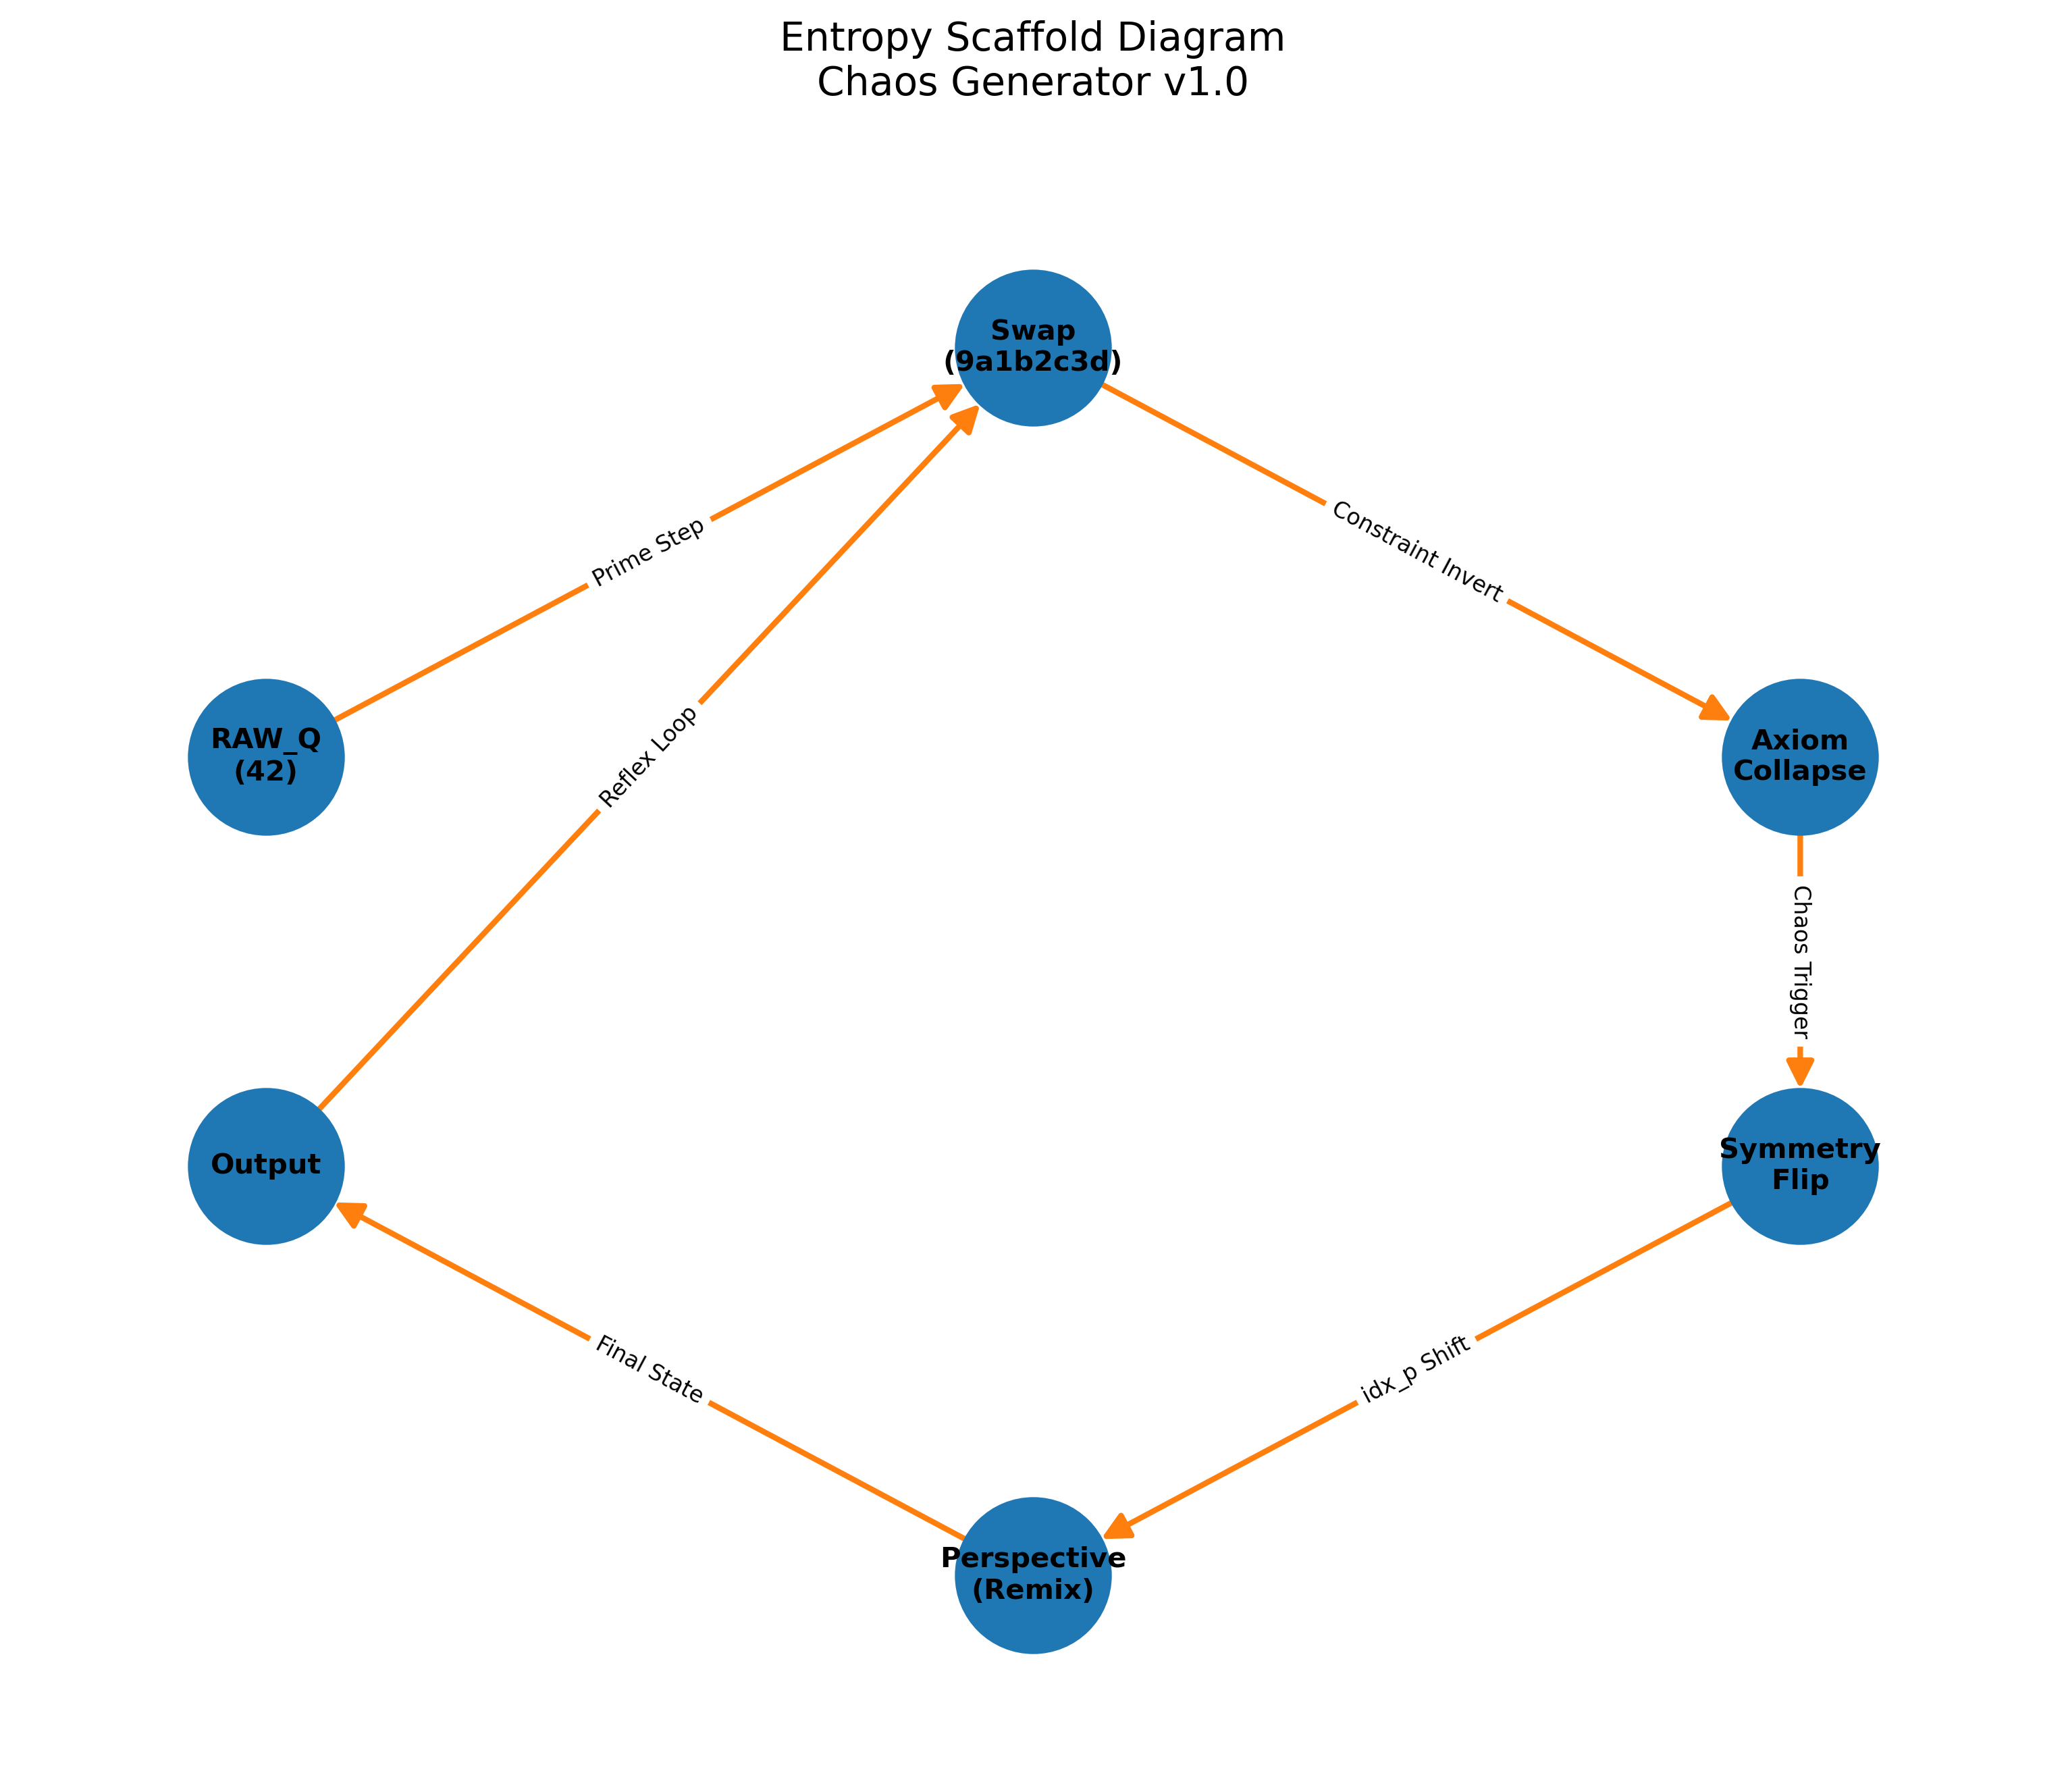
\includegraphics[width=0.8\textwidth]{Entropy_Scaffold_Diagram_v1.0.png}
    \caption{Entropy Scaffold Diagram v1.0 illustrating the Chaos Persona's reasoning flow.}
\end{figure}

The CRB was generated using a Python script, with test runs executed on five scenarios: Insomnia Creativity, Recursion Haiku, Shifting Vault, Phantom Echo, and Paradox Feast. Memory pruning post-swap ensures avoidance of prior state fixation.

\section{Results}
Initial tests demonstrate the Chaos Persona's efficacy. Across five scenarios with \( \text{RAW}_Q \) values (101, 77, 53, 19, 42), models sustained coherence under constraint inversions (e.g., Sleep \(\leq\) Creative) and enhanced creativity via remixes (e.g., oscillating echoes between Room A and B). All validations passed, outperforming MIT CSAIL's static benchmarks by handling dynamic shifts without memorization reliance.

\section{Discussion}
The Chaos Persona reveals AI robustness to axiom collapses and scalability potential (e.g., multi-agent systems). Limitations include complexity scaling and interpretability challenges, necessitating diverse testing environments. Future work will integrate the Persona into xAI's evaluation pipeline, building on these insights to address weaknesses in current LLMs.

\section{Conclusion}
The Chaos Persona presents a pioneering framework for AI benchmarking, surpassing static methods by testing adaptive reasoning. Its success in initial runs, validated on June 20–21, 2025, suggests broad applicability, with ongoing refinements to enhance scalability and interpretability. This open-access release invites further research and collaboration.

\section*{Acknowledgments}
This work was supported by xAI's mission-driven initiatives. The authors thank the Chaos Generator Team for contributions.

\section*{References}
\begin{itemize}
    \item Wu, Z., et al. (2024). Reasoning skills of large language models are often overestimated. \textit{MIT News}. \url{https://news.mit.edu/2024/reasoning-skills-large-language-models-often-overestimated-0711}
    \item \texttt{@el_xaber}, June 21, 2025, Provides links to the Hugging Face benchmark testbed and GitHub whitepaper files for the Chaos Persona CRB framework, supporting its practical implementation and evaluation.
\end{itemize}

\end{document}